%%%%%%%%%%%%%%%%%%%%%%%%%%%%%%%%%%%%%%%%%
% Beamer Presentation
% LaTeX Template
% Version 1.0 (10/11/12)
%
% This template has been downloaded from:
% http://www.LaTeXTemplates.com
%
% License:
% CC BY-NC-SA 3.0 (http://creativecommons.org/licenses/by-nc-sa/3.0/)
%
%%%%%%%%%%%%%%%%%%%%%%%%%%%%%%%%%%%%%%%%%

%------------------------------------------------------------------------------------------------
% PACKAGES AND THEMES
%------------------------------------------------------------------------------------------------

\documentclass[table, xcolor = {dvipsnames}, 9pt]{beamer}
\usepackage{tikz}
\usetikzlibrary{calc}
\usetikzlibrary{positioning}
\usetikzlibrary{arrows.meta}
\usetikzlibrary{external}
\mode<presentation> {

% The Beamer class comes with a number of default slide themes
% which change the colors and layouts of slides. Below this is a list
% of all the themes, uncomment each in turn to see what they look like.

\usetheme{default}
%\usetheme{AnnArbor}
%\usetheme{Antibes}
%\usetheme{Bergen}
%\usetheme{Berkeley}
%\usetheme{Berlin}
%\usetheme{Boadilla}
%\usetheme{CambridgeUS}
%\usetheme{Copenhagen}
%\usetheme{Darmstadt}
%\usetheme{Dresden}
%\usetheme{Frankfurt}
%\usetheme{Goettingen}
%\usetheme{Hannover}
%\usetheme{Ilmenau}
%\usetheme{JuanLesPins}
%\usetheme{Luebeck}
%\usetheme{Madrid}
\usetheme{metropolis}
%\usetheme{Malmoe}
%\usetheme{Marburg}
%\usetheme{Montpellier}
%\usetheme{PaloAlto}
%\usetheme{Pittsburgh}
%\usetheme{Rochester}
%\usetheme{Singapore}
%\usetheme{Szeged}
%\usetheme{Warsaw}

% As well as themes, the Beamer class has a number of color themes
% for any slide theme. Uncomment each of these in turn to see how it
% changes the colors of your current slide theme.

%\usecolortheme{albatross}
%\usecolortheme{beaver}
%\usecolortheme{beetle}
%\usecolortheme{crane}
%\usecolortheme{dolphin}
%\usecolortheme{dove}
%\usecolortheme{fly}
%\usecolortheme{lily}
%\usecolortheme{orchid}
%\usecolortheme{rose}
\usecolortheme{seagull}
%\usecolortheme{seahorse}
%\usecolortheme{whale}
%\usecolortheme{wolverine}
\usefonttheme{professionalfonts}
%\setbeamertemplate{footline} % To remove the footer line in all slides uncomment this line
%\setbeamertemplate{footline}[page number] % To replace the footer line in all slides with a simple slide count uncomment this line

%\setbeamertemplate{navigation symbols}{} % To remove the navigation symbols from the bottom of all slides uncomment this line
}

\usepackage{graphicx} % Allows including images
\usepackage{booktabs} % Allows the use of \toprule, \midrule and \bottomrule in tables
\usepackage{tikz}
\usepackage{multirow}
\usepackage{natbib}
\usepackage{hyperref}
\usepackage{diagbox}
\usepackage{makecell}
\usepackage{xparse}
\usepackage{subfig}
\usepackage{amsmath}
\usepackage{amsfonts,amsthm,amsmath,amssymb}    
\usepackage{bbm}
\usepackage{bm}
\usepackage{empheq}
\usepackage{pgfplots}
\usepackage{animate}
\usepgfplotslibrary{colorbrewer}

\newcommand\mybox[2][]{\tikz[overlay]\node[fill=lightgray,inner sep=2pt, anchor=text, rectangle, rounded corners=1mm,#1] {#2};\phantom{#2}}
\hypersetup{unicode=true,
            bookmarksnumbered=true,
            bookmarksopen=true,
            bookmarksopenlevel=2,
            breaklinks=false,
            pdfborder={0 0 1},
            hypertexnames=false,
            pdfstartview={XYZ null null 1}}
\usepackage{xcolor}
\newcommand\myheading[1]{%
  \par\bigskip
  {\Large\bfseries#1}\par\smallskip}
\newcommand\given[1][]{\:#1\vert\:}
\theoremstyle{plain}
\newtheorem{thm}{Theorem}
\newtheorem{prop}{Proposition\thisthmnumber}
\newtheorem{lem}{Lemma\thisthmnumber}
\newtheorem{cor}{Corollary}
\newtheorem{defin}{Definition}
\newtheorem{algo}{Algorithm}
\newcommand*\diff{\mathop{}\!\mathrm{d}}
\newcommand*\Diff[1]{\mathop{}\!\mathrm{d^#1}}
\newcommand{\bh}[1]{{\color{blue}{#1}}}
\newcommand{\mh}[1]{{\color{magenta}{#1}}}
\newcommand{\thisthmnumber}{}
\newcommand{\tikzmark}[1]{\tikz[baseline,remember picture] \coordinate (#1) {};}
\newcommand*{\QEDA}{\hfill\ensuremath{\blacksquare}}%
\newcommand*{\QEDB}{\hfill\ensuremath{\square}}%
\DeclareMathOperator{\E}{\rm{E}}
\DeclareMathOperator{\R}{\mathbb{R}}
\DeclareMathOperator{\N}{\mathbb{N}}
\DeclareMathOperator{\Var}{\rm{Var}}
\DeclareMathOperator{\Cov}{\rm{Cov}}
\DeclareMathOperator{\Supp}{\rm{Supp}}
\DeclareMathOperator{\e}{\rm{e}}
\DeclareMathOperator{\F}{\mathcal{F}}
\DeclareMathOperator{\Z}{\mathcal{Z}}
\DeclareMathOperator{\logit}{\rm{logit}}
\DeclareMathOperator{\indep}{{\perp\!\!\!\perp}}
\DeclareMathOperator{\rank}{rank}
\DeclareMathOperator*{\argmin}{arg\,min}
\DeclareMathOperator*{\argmax}{arg\,max}
%\DeclareMathOperator{\Pr}{\rm{Pr}}
%------------------------------------------------------------------------
% TITLE PAGE
%-----------------------------------------------------------------------
\pagestyle{empty}
\title[]{Randomized Experiments and Potential Outcomes} % The short title appears at the bottom of every slide, the full title is only on the title page

\author{Thomas Leavitt} % Your name
\institute[] % Your institution as it will appear on the bottom of every slide, may be shorthand to save space
{
% Your institution for the title page
\medskip
\textit{} % Your email address
}
\date{\today} % Date, can be changed to a custom date

\begin{document}

\begin{frame}
\titlepage % Print the title page as the first slide
\end{frame}

%\begin{frame}
%\frametitle{Overview} % Table of contents slide, comment this block out to remove it
%\tableofcontents % Throughout your presentation, if you choose to use \section{} and \subsection{} commands, these will automatically be printed on this slide as an overview of your presentation
%\end{frame}

%------------------------------------------------------------------------
% PRESENTATION SLIDES
%----------------------------------------------------------------
\section{Randomized experiments}
\begin{frame}{Centrality of randomized experiments to causal inference}
\vfill
\begin{itemize}
\item Experiments are conceptually and practically central \vfill
\item Not just any experiments, particular types, featuring control groups and random assignment \vfill
\item In many applications, these experiments are a ``methodological ideal'' \vfill
\item Shares outward manifestations of Stats 101 -- randomness, $p$-values, ``bias,'' confidence levels, etc -- but without the ideas that our data are sampled from some superpopulation, or a probabilistic data generating mechanism \vfill
\begin{itemize} \vfill
\item At least, those ideas are optional \vfill
\end{itemize} \vfill
\end{itemize} \vfill
\end{frame}
%----------------------------------------------------------------
\section{Random Assignment and Randomization-based Distributions}
\begin{frame}{An example: Fisher's ``Lady Tasting Tea''}
\vfill
\citet[][pp. 13-14]{fisher1935a} describes his lady tasting tea experiment as follows: \vfill
\begin{quote}
A lady declares that by tasting a cup of tea made with milk she can discriminate whether the milk or the tea infusion was first added to the cup. ... \mh{Our experiment consists in mixing eight cups of tea, four in one way and four in the other, and presenting them to the subject for judgment in a random order.} The subject has been told in advance of what the test will consist, namely that she will be asked to taste eight cups, that these shall be four of each kind, and that they shall be presented to her in a random order, that is in an order not determined arbitrarily by human choice, but by \mh{the actual manipulation of the physical apparatus used in games of chance, cards, dice, roulettes, etc., or, more expeditiously, from a published collection of random sampling numbers purporting to give the actual results of such manipulation.} Her task is to divide the 8 cups into two sets of 4, agreeing, if possible, with the treatments received.
\end{quote} \vfill
\end{frame}
%---------------------------------------------------------------
\begin{frame}{Random assignment}
\vfill
\begin{itemize} \vfill
  \item Treatment Assignment Mechanism \vfill
  \item[] \mh{Complete randomization}: Exactly $n_T$ units are treated (milk-first) and $n - n_T = n_C$ units are untreated (tea-first) \vfill
  \end{itemize} \vfill
As \citet{fisher1935a} describes: There are $\binom{8}{4} = \frac{8!}{4!(8 - 4)!} = 70$ possible ways to order $8$ cups with $4$ in milk-first condition and remaining $4$ in tea-first condition \vfill
\begin{equation}
\Omega = \left\{
\begin{bmatrix} 1 \\ 1 \\ 1 \\ 1 \\ 0 \\ 0 \\ 0 \\ 0 \end{bmatrix},
\begin{bmatrix} 1 \\ 1 \\ 1 \\ 0 \\ 1 \\ 0 \\ 0 \\ 0 \end{bmatrix},
\begin{bmatrix} 1 \\ 1 \\ 1 \\ 0 \\ 0 \\ 1 \\ 0 \\ 0 \end{bmatrix},
\cdots ,
\begin{bmatrix} 0 \\ 0 \\ 0 \\ 1 \\ 1 \\ 0 \\ 1 \\ 1 \end{bmatrix},
\begin{bmatrix} 0 \\ 0 \\ 0 \\ 1 \\ 0 \\ 1 \\ 1 \\ 1 \end{bmatrix},
\begin{bmatrix} 0 \\ 0 \\ 0 \\ 0 \\ 1 \\ 1 \\ 1 \\ 1 \end{bmatrix}
\right\}
\end{equation} \vfill
\end{frame}
%---------------------------------------------------------------
\begin{frame}{Random assignment}
\vfill
\begin{itemize} \vfill
  \item Denote each assignment in $\Omega$ by $\bm{z}^{\top} = \begin{bmatrix} z_1 & z_2 & \dots & z_n \end{bmatrix}$, \vfill \\ where $z_i = 0$ or $z_i = 1$ for all $i = 1, \ldots , n$ \vfill
  \item Due to random assignment, $\Pr\left(\mathbf{Z} = \mathbf{z} \right) = \left\lvert \Omega \right\rvert^{-1}$ \vfill
\begin{itemize} \vfill
\item[] In general $\left\lvert S \right\rvert$ denotes the ``cardinality'' of (i.e., the number of elements in) the set $S$ \vfill
 \end{itemize} \vfill
 \item So in Fisher's ``Lady Tasting Tea'' experiment, each allocation of $8$ cups to $4$ milk-first and $4$ tea-first conditions has probability $(1/70)$ \vfill
 \begin{equation}
\Pr\left(\bm{Z} = \bm{z}\right) = \dfrac{1}{70} \text{ for all } \bm{z} \in \Omega
 \end{equation} \vfill
  \end{itemize} \vfill
\end{frame}
%---------------------------------------------------------------
\begin{frame}{Randomization-based distributions}
\vfill
\begin{itemize}
\item Suppose that among $70$ assignments, the $1$st happened to be randomly selected \vfill
\item When presented with randomly selected ordering of $8$ cups, the ``lady'' correctly identifies all $4$ milk-first and all $4$ tea-first cups \vfill
\vspace{1em}
\begin{table}[H]
\centering
\begin{tabular}{l|cc}
\toprule
Unit & $\bm{z}$ & $\bm{y}$ \\ 
  \midrule
$1$ & $1$ & $1$  \\ 
$2$ & $1$ & $1$  \\ 
$3$ & $1$ & $1$  \\ 
$4$ & $1$ & $1$  \\ 
$5$ & $0$ & $0$  \\ 
$6$ & $0$ & $0$  \\ 
$7$ & $0$ & $0$ \\ 
$8$ & $0$ & $0$ 
\end{tabular}
\caption{Results of R. A. Fisher's ``Lady Tasting Tea'' experiment}
\label{tab: lady tasting tea obs data}
\end{table}
\vspace{-2em}
\vfill
\item We can summarize realized data by number of focal-group (milk-first) cups correctly identified as such, $\mathbf{z}^{\top}\mathbf{y}$, which in this case is equal to $4$ \vfill
\end{itemize}
\end{frame}
%---------------------------------------------------------------
\begin{frame}{Randomization-based distributions}
\vfill
\begin{itemize} \vfill
\item \citet{fisher1935a} showed that we can entertain \mh{counter-to-fact assignments of treatment}, holding responses fixed at their observed values \vfill
\item This fits notion that ``lady'' cannot discriminate between milk-first and tea-first \vfill
\end{itemize} \vfill 
\begin{table}[H]
\scriptsize
    \begin{tabular}{l|l}
    \toprule
    $\mathbf{z}_1$ & $\mathbf{y}$ \\ \midrule
    1 & 1  \\
    1 & 1   \\
    1 & 1   \\
    1 & 1  \\
    0 & 0  \\
    0 & 0  \\
    0 & 0  \\
    0 & 0  
    \end{tabular}
    \hfill
      \begin{tabular}{l|l}
      \toprule
    $\mathbf{z}_2$ & $\mathbf{y}$ \\ \midrule
    1 &  1  \\
    1 &  1  \\
    1 &  1  \\
    0 &  1   \\
    1 &  0  \\
    0 &  0  \\
    0 &  0  \\
    0 &  0  
    \end{tabular}
     \hfill
      \begin{tabular}{l|l}
      \toprule
    $\mathbf{z}_3$ & $\mathbf{y}$ \\ \midrule
    1 & 1  \\
    1 & 1  \\
    1 & 1  \\
    0 & 1   \\
    0 & 0  \\
    1 & 0  \\
    0 & 0  \\
    0 & 0  
    \end{tabular}
     \hfill
     $\cdots $
     \hfill
      \begin{tabular}{l|l}
      \toprule
    $\mathbf{z}_{68}$ & $\mathbf{y}$ \\ \midrule
    0 & 1  \\
    0 & 1  \\
    0 & 1  \\
    1 & 1   \\
    1 & 0  \\
    0 & 0  \\
    1 & 0  \\
    1 & 0  
    \end{tabular}
     \hfill
      \begin{tabular}{l|l}
      \toprule
    $\mathbf{z}_{69}$ & $\mathbf{y}$ \\ \midrule
    0 & 1  \\
    0 & 1  \\
    0 & 1  \\
    1 & 1  \\
    0 & 0 \\
    1 & 0  \\
    1 & 0  \\
    1 & 0  
    \end{tabular}
     \hfill
      \begin{tabular}{l|l}
      \toprule
    $\mathbf{z}_{70}$ & $\mathbf{y}$ \\ \midrule
    0 & 1  \\
    0 & 1  \\
    0 & 1  \\
    0 & 1  \\
    1 & 0   \\
    1 & 0  \\
    1 & 0  \\
    1 & 0  
    \end{tabular}
    \caption{Possible realizations of data holding observed outcomes fixed}
\label{tab: fisher's null pot outs schedule}
\end{table}
\end{frame}
%---------------------------------------------------------------
\begin{frame}{Randomization-based distributions}
\vfill
\begin{itemize} \vfill
\item \citet{fisher1935a} showed that we can derive distribution of test-statistic under this claim that ``lady'' cannot discriminate between milk-first and tea-first \vfill
\end{itemize}  \vfill
\begin{figure}[H]
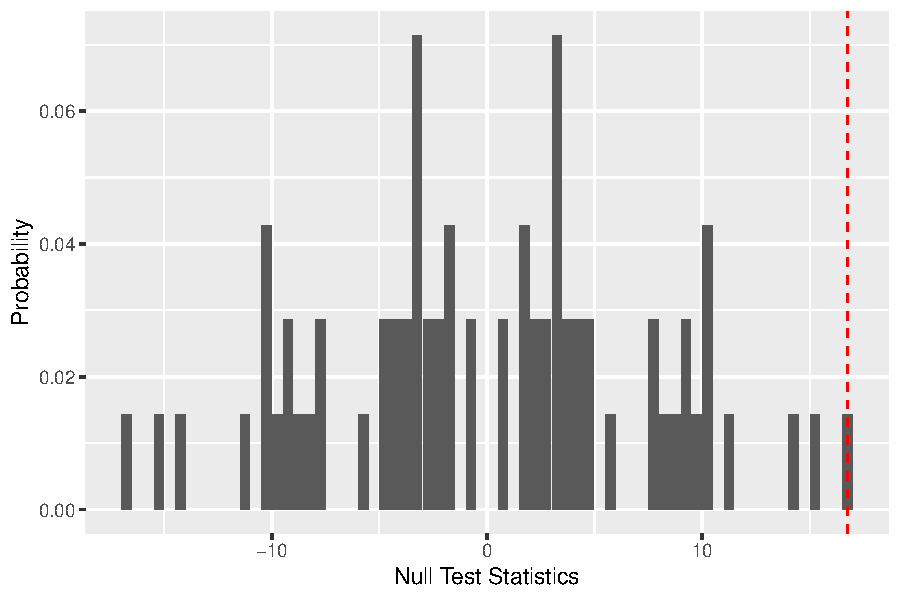
\includegraphics[width=0.9\linewidth]{null_dist_plot.pdf}
\caption{Distribution of test-statistic over assignments holding outcomes fixed at observed values}
\end{figure} \vfill
\end{frame}
%---------------------------------------------------------------
\section{Potential Outcomes}
\begin{frame}{Potential outcomes}
\vfill
\begin{itemize} \vfill
\item Thus far, we have entertained counter-to-fact assignments of treatment, holding responses fixed at their observed values \vfill
\item \citet{neyman1923} and \citet{rubin1974} also posited unobserved, counter-to-fact \mh{potential outcomes} \vfill
\item In ``Lady Tasting Tea'' example, we can imagine other responses to possible treatments in which observed outcomes are \textit{not} fixed \vfill
\begin{itemize} \vfill
\item E.g., perfect discrimination \vfill
\end{itemize} \vfill
\vspace{2em}
\begin{table}[H]
\scriptsize
    \begin{tabular}{l|l}
    \toprule
    $\mathbf{z}_1$ & $\mathbf{y}$ \\ \midrule
    1 & 1  \\
    1 & 1   \\
    1 & 1   \\
    1 & 1  \\
    0 & 0  \\
    0 & 0  \\
    0 & 0  \\
    0 & 0  
    \end{tabular}
    \hfill
      \begin{tabular}{l|l}
      \toprule
    $\mathbf{z}_2$ & $\mathbf{y}$ \\ \midrule
    1 &  1  \\
    1 &  1  \\
    1 &  1  \\
    0 &  0   \\
    1 &  1  \\
    0 &  0  \\
    0 &  0  \\
    0 &  0  
    \end{tabular}
     \hfill
      \begin{tabular}{l|l}
      \toprule
    $\mathbf{z}_3$ & $\mathbf{y}$ \\ \midrule
    1 & 1  \\
    1 & 1  \\
    1 & 1  \\
    0 & 0   \\
    0 & 0  \\
    1 & 1  \\
    0 & 0  \\
    0 & 0  
    \end{tabular}
     \hfill
     $\cdots $
     \hfill
      \begin{tabular}{l|l}
      \toprule
    $\mathbf{z}_{68}$ & $\mathbf{y}$ \\ \midrule
    0 & 0  \\
    0 & 0  \\
    0 & 0  \\
    1 & 1   \\
    1 & 1  \\
    0 & 0  \\
    1 & 1  \\
    1 & 1  
    \end{tabular}
     \hfill
      \begin{tabular}{l|l}
      \toprule
    $\mathbf{z}_{69}$ & $\mathbf{y}$ \\ \midrule
    0 & 0  \\
    0 & 0  \\
    0 & 0  \\
    1 & 1  \\
    0 & 0 \\
    1 & 1  \\
    1 & 1  \\
    1 & 1  
    \end{tabular}
     \hfill
      \begin{tabular}{l|l}
      \toprule
    $\mathbf{z}_{70}$ & $\mathbf{y}$ \\ \midrule
    0 & 0  \\
    0 & 0  \\
    0 & 0  \\
    0 & 0  \\
    1 & 1   \\
    1 & 1  \\
    1 & 1  \\
    1 & 1  
    \end{tabular}
    \caption{Possible realizations of data under perfect discrimination}
\label{tab: fisher's perfect discrim pot outs schedule}
\end{table} \vfill
\end{itemize}  
\vfill
\end{frame}
%---------------------------------------------------------------
\begin{frame}{Potential outcomes}
\vfill
\begin{figure}[H]
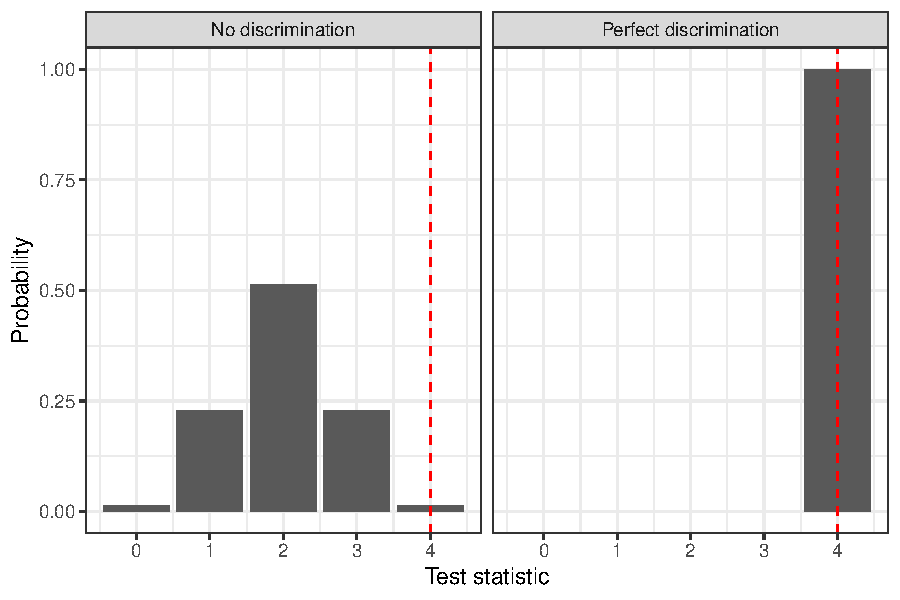
\includegraphics[width=0.9\linewidth]{perfect_discrim_test_stat_plot.pdf}
\caption{Distribution of test-statistic over assignments for different potential outcomes schedules}
\end{figure} \vfill
\end{frame}
%---------------------------------------------------------------
\begin{frame}{Potential outcomes}
\vfill
\begin{itemize} \vfill
\item A \mh{potential outcomes schedule} is vector-valued function $\bm{y}: \Omega \mapsto \R^n$ \vfill
\item Intuitively, a listing of how each study participant would respond to any $\bm{z} \in \Omega$ that a random assignment process could produce \vfill
\item We usually consider potential outcomes schedules that satisfy Stable Unit Treatment Value Assumption (SUTVA) \citep{cox1958a,rubin1980b,rubin1986}: \vfill
\item SUTVA means that \vfill
\begin{enumerate} \vfill
\item Units in experiment respond to only treatment condition to which each unit is individually assigned \vfill
\item Treatment condition is actually the same treatment for all units assigned to treatment and control condition is the same for all units assigned to control \vfill
\end{enumerate} \vfill
\end{itemize}  
\vfill
\end{frame}
%---------------------------------------------------------------
\begin{frame}{Potential outcomes}
\vfill
\begin{itemize} \vfill
\item Under SUTVA, write potential outcomes for unit $i$ as $y_{Ti}$ or $y_{Ci}$ \vfill
\item One fixed value of the outcome for unit $i$ if it is assigned to treatment and another fixed value of unit $i$ if it is assigned to control \vfill
\item Consider unit $i = 4$ of perfect discrimination potential outcomes schedule: \vfill
\vspace{1em}
\begin{table}[H]
\scriptsize
    \begin{tabular}{l|l}
    $\mathbf{z}_1$ & $\mathbf{y}$ \\ \midrule
    1 & 1  \\
    1 & 1   \\
    1 & 1   \\
    \mh{1} & \mh{1}  \\
    0 & 0  \\
    0 & 0  \\
    0 & 0  \\
    0 & 0  
    \end{tabular}
    \hfill
      \begin{tabular}{l|l}
    $\mathbf{z}_2$ & $\mathbf{y}$ \\ \midrule
    1 &  1  \\
    1 &  1  \\
    1 &  1  \\
    \mh{0} &  \mh{0}   \\
    1 &  1  \\
    0 &  0  \\
    0 &  0  \\
    0 &  0  
    \end{tabular}
     \hfill
      \begin{tabular}{l|l}
    $\mathbf{z}_3$ & $\mathbf{y}$ \\ \midrule
    1 & 1  \\
    1 & 1  \\
    1 & 1  \\
    \mh{0} & \mh{0}   \\
    0 & 0  \\
    1 & 1  \\
    0 & 0  \\
    0 & 0  
    \end{tabular}
     \hfill
     $\cdots $
     \hfill
      \begin{tabular}{l|l}
    $\mathbf{z}_{68}$ & $\mathbf{y}$ \\ \midrule
    0 & 0  \\
    0 & 0  \\
    0 & 0  \\
    \mh{1} & \mh{1}   \\
    1 & 1  \\
    0 & 0  \\
    1 & 1  \\
    1 & 1  
    \end{tabular}
     \hfill
      \begin{tabular}{l|l}
    $\mathbf{z}_{69}$ & $\mathbf{y}$ \\ \midrule
    0 & 0  \\
    0 & 0  \\
    0 & 0  \\
    \mh{1} & \mh{1}  \\
    0 & 0 \\
    1 & 1  \\
    1 & 1  \\
    1 & 1  
    \end{tabular}
     \hfill
      \begin{tabular}{l|l}
    $\mathbf{z}_{70}$ & $\mathbf{y}$ \\ \midrule
    0 & 0  \\
    0 & 0  \\
    0 & 0  \\
    \mh{0} & \mh{0}  \\
    1 & 1   \\
    1 & 1  \\
    1 & 1  \\
    1 & 1  
    \end{tabular}
    \caption{Possible realizations of data under perfect discrimination}
\end{table} \vfill
\item Each unit has at most two potential outcomes \vfill
\end{itemize}  
\vfill
\end{frame}
%---------------------------------------------------------------
\begin{frame}{Potential outcomes}
\vfill
\begin{itemize} \vfill
\item \mh{Fundamental Problem of Causal Inference} \citep{holland1986}: \vfill
  \begin{center}
    We can never observe both $y_{Ti}$ and $y_{Ci}$ for the same $i$\\
  \end{center} \vfill
\item We can observe only one of the two potential outcomes:
  $$ Y_i = Z_i y_{Ti} + (1 - Z_i)y_{Ci}$$ \vfill
\end{itemize}  
\vfill
\end{frame}
%---------------------------------------------------------------
\section{For next time ... }
\begin{frame}{Causal Inference}
\vfill
\begin{itemize} \vfill
\item Given this setup of random assignment and potential outcomes schedules \vfill
\begin{center}
\mh{What statistical tools can we use to assess evidence against No Discrimination and in favor of Perfect Discrimination (or vice versa)?}
\end{center}
\vfill
\end{itemize} \vfill
\end{frame}
%---------------------------------------------------------------

\begin{frame}
\frametitle{References} 
\scriptsize
\bibliographystyle{chicago}
\bibliography{Master_Bibliography}   % name your BibTeX data base
\end{frame}
%---------------------------------------------------------------
\end{document}